\documentclass[10pt,journal,compsoc]{IEEEtran}
\usepackage{subfiles}
\usepackage[pdftex]{graphicx}
\usepackage{amsmath}
\usepackage{xspace}
\usepackage{multirow}
\usepackage{amssymb}
\usepackage{algorithm}
\usepackage[noend]{algpseudocode}
\renewcommand{\algorithmicrequire}{\textbf{Input:~}}
\renewcommand{\algorithmicensure}{\textbf{Output:~}}
\newcommand\ovr[1]{\overrightarrow{#1}}

\usepackage{array}
\usepackage{color}
\usepackage{listings}
\usepackage{placeins}
\usepackage{enumitem}


\ifCLASSOPTIONcompsoc
  \usepackage[nocompress]{cite}
\else
  \usepackage{cite}
\fi

\ifCLASSINFOpdf
\else
\fi

\newcommand\MYhyperrefoptions{bookmarks=true,bookmarksnumbered=true,
pdfpagemode={UseOutlines},plainpages=false,pdfpagelabels=true,
colorlinks=true,linkcolor={black},citecolor={black},urlcolor={black},
pdftitle={Bare Demo of IEEEtran.cls for Computer Society Journals},%<!CHANGE!
pdfsubject={Typesetting},%<!CHANGE!
pdfauthor={Michael D. Shell},%<!CHANGE!
pdfkeywords={Computer Society, IEEEtran, journal, LaTeX, paper,
             template}}%<^!CHANGE!


\begin{document}

\title{Fast Influence Maximization Sketching\\ with Fusing and Vectorization }


\author{G\"{o}khan~G\"{o}kt\"{u}rk
        and~Kamer~Kaya% <-this % stops a space
\IEEEcompsocitemizethanks{\IEEEcompsocthanksitem G. G\"{o}kt\"{u}rk and K. Kaya are with Computer Science and Engineering, Faculty of Engineering and Natural Sciences, Sabanci University, Istanbul, Turkey.}% <-this % stops a space
%\thanks{Manuscript received April 19, 2005; revised August 26, 2015.}}
}
%FIXME



\markboth{Journal of \LaTeX\ Class Files,~Vol.~14, No.~8, August~2015}%
{Shell \MakeLowercase{\textit{et al.}}: Bare Advanced Demo of IEEEtran.cls for IEEE Computer Society Journals}


\IEEEtitleabstractindextext{%
\begin{abstract}
The abstract goes here.
\end{abstract}

% Note that keywords are not normally used for peerreview papers.
\begin{IEEEkeywords}
Computer Society, IEEE, IEEEtran, journal, \LaTeX, paper, template.
\end{IEEEkeywords}}


\maketitle

\IEEEdisplaynontitleabstractindextext
\IEEEpeerreviewmaketitle


\ifCLASSOPTIONcompsoc
\IEEEraisesectionheading{\section{Introduction}\label{sec:introduction}}
\else
\section{Introduction}
\label{sec:introduction}
\fi

Influence maximization is the problem of finding subset of $K$ vertices in a graph $G$ that has maximum reachability on some diffusion model $M$. 

In addition to introducing the problem, Kempe et al.\cite{kempe2003maximizing} proved it to be NP-hard and provided a greedy Monte-Carlo approach that has a constant approximation for the optimal solution.




Many heuristics and proxy methods have been proposed in the literature~\cite{MixGreedy, narayanam2010shapley, kimura2007extracting, chen2010PMIA,chen2010LDAG, kim2013scalable, skim, goyal2011simpath, jung2012irie,cheng2014imrank,liu2014influence,galhotra2016holistic}.


\section{Notation and Background}\label{sec:background}

We denoted $G = (V,E)$ as a directed graph where the $n$ vertices in $V$ represent the agents, and $m$ edges in $E$ represent the relations between the agents in $V$.
The neighborhood of a vertex $u \in V$ is denoted as $\Gamma_G(v) = \{v: (u,v) \in E\}$. 
A graph $G' = (V',E')$ is a subgraph of $G$ if $V' \subseteq V$ and $E' \subseteq E$. 
Diffusion probability on edge $(u, v) \in G$ is noted as $w_{u,v}$.
$w_{u,v}$ can be determined either by the diffusion model or according to the strength of $u$ and $v$'s relationship in the data.

\begin{table}[!ht]
    \caption{Table of notations}
    \label{tab:notation}
    \centering
    \begin{tabular}{|l|p{0.7\linewidth}|}
        \hline
        Variable & Definition  \\
        \hline
        $G = (V,E)$     & Graph $G$ with vertices $V$ and edges $E$ \\
        $\Gamma_G(v)$   & Neighborhood of vertex $v$ in graph $G$\\
        $w_{u,v}$       & Probability of $u$ directly influencing $v$ \\
        %$SCC(v) $       & Strongly connected component of vertex $v$\\
        $R_{G}(v)$      & Reachability set of vertex $v$ on graph $G$\\
%        $\overline{R_{G}(v)} & Complement of the vertex set $R_{G}(v)$\\
        \hline\hline
        $S$             & Seed set to maximize influence\\
        $K$             & Size of the seed set\\
        $\mathcal{R}$   & Number of Monte-Carlo simulations performed\\
        $\sigma_{G}(S)$ & Influence score of $S$ in $G$, i.e., expected number of vertices reached from $S$ in $G$\\
        % $\sigma_{G}{(S,v)}$          & Marginal influence gain by adding vertex $v$ to seed set $S$\\
\hline\hline
        %$p$             & Sampling probability for edges\\
%        $P(s,v)_r $     & Random probability generated for selecting edge vertices $s$ to $v$ in simulation $r$\\
        $h(u,v)$        & Hash function for edge $\{u,v\}$\\
        $h_{max}$       & Maximum value hash function $h$ can return\\
        %$X_r$           & Random number/hash generated for simulation $r$  \\
        \hline\hline
        $B$             & Batch size, number of simultaneous simulations ran.\\
        $e$             & Estimated reachability set size\\
        % $[a, \ldots, a]_B$      & Vector of size $B$, contains all $a$\\
        $M_u[j]$        & Sketch $j$th register for vertex $u$\\
        $\varsigma $    & Influence gained before sketch build\\
        $\sigma $       & Influence Score\\
        $\delta$        & Marginal Gain after sketch build\\
        $\epsilon_g$    & Allowed global estimation error ratio\\
        $\epsilon_l$    & Allowed local estimation error\\ 
        $\epsilon_c$    & Allowed non-convergenced vertex ratio\\
      %  $x[[i, j]]$   & Slice of vector  $x$ between indices $i$ and $j$, not including $j$ \\ 
        \hline         
    \end{tabular}
\end{table}
\subsection{Influence Maximization}

Influence Maximization aims to find a seed set $S \subseteq V$ among all possible size $K$ subsets of $V$ that maximizes an {\em influence spread function} $\sigma$  when the diffusion process is initiated from $S$. Although we focus on undirected graphs, for IM, the graph can be directed or undirected depending on the initial construction. Figure~\ref{fig:xx} shows a~(Fig.~\ref{fig:ic}) and directed~(Fig.~\ref{fig:wc})
graph for which the weights on the edges are diffusion/influence probabilities. 

\begin{figure}[!ht] 
    \centering
  \subfloat[\small{IC}\label{fig:ic}]{%
       \includegraphics[width=0.45\linewidth]{ic-dif.png}}
  \subfloat[\small{WC}\label{fig:wc}]{%
        \includegraphics[width=0.45\linewidth]{wc-dif.png}}
    \\% IMAGES HERE
  \caption{\protect\subref{fig:ic} 
The directed graph $G = (V, E)$ for Independent Cascade with independent diffusion probabilities. 
\protect\subref{fig:wc}
The directed graph obtained from the directed one by setting the diffusion probabilities of incoming edges to $1 / |\Gamma_G(v)|$ for each vertex $v \in V$. 
  }
  %\label{fig_ic_model} 
  \label{fig:xx} 
\end{figure}
The influence spread function $\sigma_{G,M}(\cdot)$ computes the {\em expected} number of agents/nodes/vertices influenced~(activated) through a diffusion model $M$. For the sake of simplicity, we drop $M$ from the notation; in the rest of the text, $\sigma_{G}$ refers to $\sigma_{G,M}$. Some of the popular diffusion models for IM in the literature are {\em independent} and {\em weighted cascade}~(IC and WC),  and {\em linear threshold}~(LT)~\cite{kempe2003maximizing}. 


\subsection{Sketch}\label{sec:sketch}
The count-distinct problem is the problem of finding the number of distinct elements in a stream with non-distinct elements. Computing reachability sets of a vertex is a similar problem; cardinality of all vertices visited is calculated while traversing sample sub-graphs from the given vertex. Exact cardinality calculations requires memory proportional to the cardinality. 

Reachability set of a vertex is distinct union of all connected vertices' reachability sets. Many other Influence Maximization methods exploit this property in some degree. 

The methods based on Reverse reachability and Bottom-Up Traversal, utilizes this property directly to merge reachability sets of connected vertices to estimate vertices influence.
MixGreedy method goes one step further; it utilizes that all vertices in a connected component that have the same reachability set in undirected graphs. So that, for a sample graph, all reachability sets can be found in single graph traversal. 

For directed graphs, storing reachability sets for all vertices and merging these sets are infeasible for non-trivial graphs. 
% If one-hot vectors are used to store reachability sets for constant insertion time, $O(n^2\mathcal{R})$ bits of memory is required and each merge operation has $O(n)$ time complexity. 
if Disjoints sets are used for storing reachability sets; $(n\bar{\sigma}\mathcal{R})$ memory is required to store all reachability sets, and each merge operation has $O(ackermann'(\sigma))$ complexity.

Count-distinct sketches have nice properties for such problems; Flajolet–Martin algorithm can estimate cardinality of distinct elements in reachability sets with constant number of registers($M$), and most importantly union of these sets can be done in constant number of operations.

Flajolet–Martin sketch only stores how rare elements are in a multi-set.Rarity of the elements are often computed by counting leading zeros in item's hash values. Items are added by storing longest leading zero count. Cardinality estimation can be done by taking 2 to the power of the stored value. Multiple registers, $M[j]$, are commonly used to reduce variance, average of longest running zeros can be used compute the cardinality and the result is divided to correction factor $\phi \approx 0.77351$ to correct hash collisions.

The merge operation for two sketches, $M_u$,$M_v$, can be performed by computing the pairwise maximum of the registers; $M[j] = max(M_u[j],M_v[j]) ~ \forall j\in(0,J]$

In this work, we utilize a variant of Flajolet–Martin sketch; since multiple Monte-Carlo simulations are performed to calculate estimated influence, we use one register per simulation, and take average of longest leading zero counts to calculate average cardinality of reachability sets. Also, in an another perspective, it is same as using register as much as MC simulation, where updates are done with same probability as influence propagation. 


\subsection{SIMD}
{\em Single Instruction-Multiple Data} machines exploits data level parallelism to perform the same operation on multiple data points simultaneously. In this work, we utilized Advanced Vector Extensions (AVX2) instruction set. AVX2 works on 256-bit registers in multiple packed forms; 8x32 bit operations are used in fused sampling, where as sketch merge  performed with 32x8bit operations. This dichotomy between operations solved by processing in 32 simulations batches at a time.
Even-though, auto-vectorization is enabled, most of the operation mention are cannot by vectorized by the used compiler. As far as we know, no compiler vectorizes chain conditional move or move-mask operations. Vectorization in the implementation is done using explicit intrinsics.

% First, active edges are checked by generating random values, $P(u,v)_r$. After comparing random values with edge threshold, active edges are store in an 32bit integer as one-hot vector. Then,  


For completeness, the intrinsics explicitly used in this paper are described in Table~\ref{tab:avx2-instructions}.

\begin{table}[!ht]
    \caption{AVX2 intrinsics used in the implementation.}
    \label{tab:avx2-instructions}
    \centering

    \begin{tabular}{|p{0.33\linewidth}|p{0.58\linewidth}|}
    \hline
    Intrinsic & Definition\\
    \hline
    {\tt \_mm256\_set1\_epi32} & Initializes 256-bit vector with scalar integer values. Doesn't map to any AVX instructions. \\
        % \hline
    {\tt \_mm256\_and\_si256} & Performs bitwise logical AND operation on 256-bit integer vectors. \\
            % \hline
    {\tt \_mm256\_xor\_si256} &  Performs bitwise logical XOR operation on 256-bit integer vectors.\\
            % \hline
    {\tt \_mm256\_cmpgt\_epi32} & Compares packed 8x 32-bit integers of two input vectors. \\
            % \hline
        % \hline
    {\tt \_mm256\_movemask\_ps} & Extracts the first bits of 8x 32-bit elements in a compact 8-bit format \\
            % \hline
    {\tt \_mm256\_blendv\_epi8} & Blends/selects byte elements of input vectors depending on the bits in a given mask vector.\\ 
             \hline         
    \end{tabular}
\end{table}{}

\section{Method}\label{sec:method}

\subsubsection{Hash-based Fused Sampling}
The probabilistic nature of cascade models requires sampling sub-graphs $\hat{G}$ from $G = (V, E)$ to simulate the diffusion process.  Sampling can be a dominating factor in processing; sampling may demand multiple passes on the graph, if samples are memoized, multiple times of the graph size needs to be stored.
In this work, samples are not generated explicitly. By using a hash-based, fused sampling, we eliminate the necessity of in-memory creation and storage of the sample sub-graphs.
While processing an edge, it is considered for all possible samples.
It is sampled or skipped depending on the outcome of hash based random value. The hash function used is given in equation \ref{eq:hash}
\begin{equation}
    \label{eq:hash}
    h(u,v) = \mbox{{\sc Murmur3}}(u||v)  
\end{equation}
where $||$ is the concatenation operator. 

The {{\sc Murmur3}}~\cite{MurmurHash3} hash function is preferred because of its simplicity, good avalanche behavior and bias$.

For performance considerations, edge hash values were pre-computed in our work and only existing pairs were considered. The trade-off between extra memory and computation here maybe not be applicable for different architectures and faster/simpler hash functions.

Although the above-mentioned approach generates a unique hash value for each edge, and hence a unique sampling probability, different simulations require different probabilities.

Multiple deterministic random values for each edge is generated by using the edge hash values and random numbers $X_r$ associated with each simulation $r$. 
Sampling probability of $(u, v)$ for simulation $r$, $P(u, v)_r$, is computed as follows; First, $h(u,v)$ is XOR'ed with a uniformly randomly chosen $X_r \in_R [0, h_{max}]$ and the result is normalized by dividing the value to the upper limit of the hash value $h_{max}$. Formally,
\begin{equation}
    \label{eq:hash_prob}
    {\rho}(u,v)_r = \frac{X_r \oplus h(u,v)}{h_{max}}.
\end{equation}

The edge $\{u,v\}$ is verified to be in the sample if ${\rho}(u,v)_r$ is smaller than or equal to the threshold $w_{u,v}$. 
The edge $\{u,v\}$ is exists in the sample $r$ if and only if  ${P}(u,v)_r$ is smaller than the edge threshold $w_{u,v}$. One of the benefits of this approach is, sampling an edge is only single XOR and compare-greater-than operations. In addition, the following control flow branch can be removed using conditional move operations. An efficient SIMD implementation of this approach will be discussed later in this section.

Using a strong hash function such as {{\sc Murmur3}} ensures all bits independently change if the input is changed. This property allows us to generate good enough pseudo-random values for fair sampling. To prove the fairness of random values generated with the hash-based approach, we generated a large number of samples for various real-life networks and graphed the Cumulative Distribution Function~(CDF) of random values $P(u,v)_r$ used while sampling.

For a given graph $G = (V,E)$, the CDF of a sampling probability $x$ is computed as $\Pr\left(x \leq P(u,v)_r\right)$ for all $(u,v) \in E$ and $0 \leq r < R$. Figure~\ref{fig:prob_cdf} shows the CDFs for 12 real-life networks. The sampling probability distribution with hash-based computation is almost identical with the uniform distribution which is used to simulate the influence diffusion process.

\begin{figure}[!ht] 
    \centering
    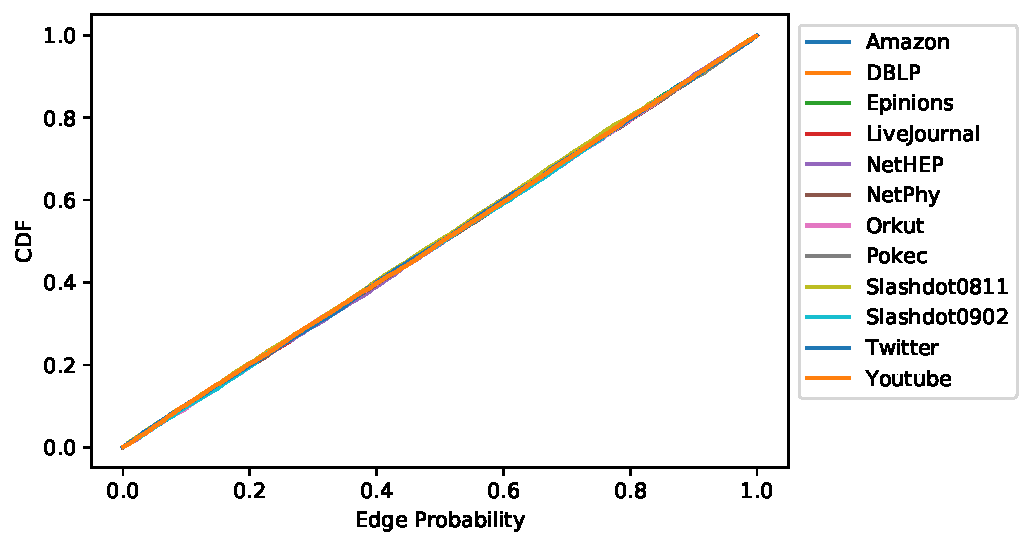
\includegraphics[width=1\linewidth]{cdf}
    \caption{Cumulative distribution function of hash-based sampling probabilities on various real-life networks.}
    \label{fig:prob_cdf} 
\end{figure}

%Traditional implementations sample each edge in $G$ once per simulation and store them to construct a sampled subgraph. n
Since it is possible to know if the edge traversed whether is in any sample, many memory access overheads are avoided. Only down-side of hash-based fused sampling is that, all probabilities $P(u,v)_r$  should be generated for each edge traversal. Fortunately, this computations are quite fast on modern computing hardware.

\subsection{Reachability Set Cardinality Estimation}

Greedy solution to influence maximization problem requires finding a vertex that maximizes marginal influence gain at each step. Until $K$ vertices are added to the seed set this procedure is repeated. 
Finding a vertex's influence is distinct element count in all sample sub-graphs. Count-distinct sketch we mentioned in section \ref{sec:sketch} is 




\begin{algorithm}
\caption{\sc{SketchFuser}($G,K,J$)}
\label{algo:newgredy}
\algorithmicrequire{$G = (V,E)$: the influence graph
\\\hspace*{6.6ex}{$K$: number of seed vertices
\\\hspace*{6.7ex}$\mathcal{J}$: number of MC simulations}\\}
\algorithmicensure{$S$: a seed set that maximizes influence on $G$
}
\begin{algorithmic}[1]
    \State {$S \leftarrow \{\emptyset\}$}
    \For{$ v\in V$}
        \For{$ j\in J$}
            \State $M[j]_v \leftarrow clz(hash(v) \oplus hash(j))$ 
        \EndFor
    \EndFor
    \State $M \leftarrow Simulate(G,M,\emptyset)$
    \State $mask \leftarrow zeros(J)$
    \State $\varsigma \leftarrow 0$
    \For{$k=1\ldots K$}
        \State $s \leftarrow \underset{v\in V}{\mathrm{argmax}} ~estimate(merge(mask,M_v))$
        \State $S \leftarrow S \cup \{s\}$
        \State $e \leftarrow estimate(merge(mask,M_s))$
        % \State $R_S \leftarrow run\_cascade(G,S,J)$
        \State {Compute seed set $S$'s Reachability set $R_S(S)$ }
        \State $\sigma_G(S) \leftarrow |R_S|/J$
        \State $\delta = \sigma - \varsigma$
        \If{$ (e - \delta) / \delta < \epsilon_l \lor |e-\delta| / \sigma < \epsilon_g$}
            \State $mask \leftarrow merge(mask,M_s)$
        \Else
            \For{$ v\in V$}
                \For{$ j\in J$}
                    \State $M[j]_v \leftarrow clz(hash(v) \oplus hash(j))$ 
                \EndFor
            \EndFor
            \State $M \leftarrow simulate(G,M,R_S)$
            \State $mask \leftarrow zeros(J) $ 
            \State $\varsigma \leftarrow \sigma $ 
        \EndIf
    \EndFor
    \State \Return $S$
\end{algorithmic}
\end{algorithm}

\begin{algorithm}
\caption{\sc{Simulate}($G,M,J,R_S$)}
\label{algo:newgredy}
\algorithmicrequire{$G = (V,E)$: the influence graph
\\\hspace*{6.6ex}{$M$: Sketch vectors of vertices
\\\hspace*{6.7ex}$\mathcal{J}$: number of MC simulations
\\\hspace*{6.7ex}$R_S$: Reachability set of the seed set
}
\\}
\algorithmicensure{$M$: Updated Sketch vectors
}
\begin{algorithmic}[1]
    \State {$L \leftarrow V$}
    \State {$L' \leftarrow {\emptyset}$}
    \While{$|L|/|V| > \epsilon_c$}
        \For{$e_{u,v} \in \Gamma(L)$} %REVERSE THIS
            \For{$j \in (0,J]$}
                \If{$P(u,v)_j < W_{u,v} \land u  \not\in R_S[j]$}
                    \State{$M_u[j]\leftarrow max(M_u[j],M_v[j])$}                
                \EndIf
            \EndFor
            \If {$M_u$ changed}
                \State $L' \cup u $
            \EndIf
        \EndFor
        \State $L \leftarrow L'$
        \State $L' \leftarrow \{\emptyset\}$
    \EndWhile
\end{algorithmic}
\end{algorithm}



\section{Evaluation}\label{sec:evaluation}

\section{Related Work}\label{sec:relatedwork}

\section{Conclusion}\label{sec:conclusion}

\ifCLASSOPTIONcaptionsoff
  \newpage
\fi


\bibliographystyle{IEEEtran}
\bibliography{refs}
\begin{IEEEbiography}[{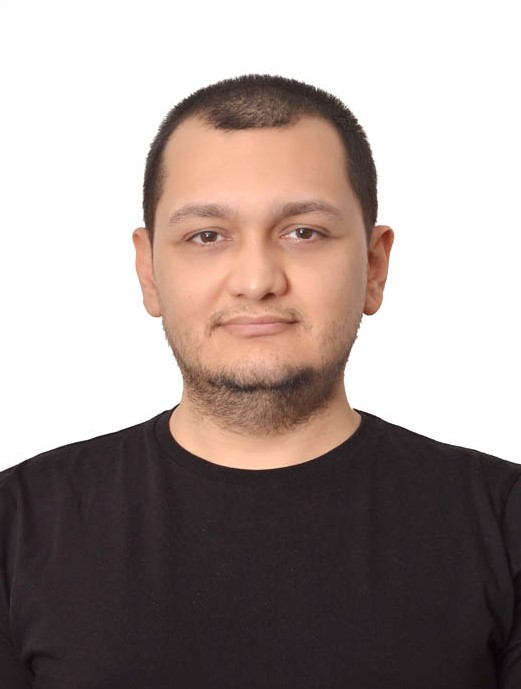
\includegraphics[width=1in,height=1.25in,clip,keepaspectratio]{./images/gokhan.png}}]{G\"{o}khan~G\"{o}kt\"{u}rk} is a PhD candidate at the Faculty of Engineering and Natural Sciences in Sabancı University. He has received his BS and MS degrees from Sabancı University as well. He is interested in High Performance Computing, Parallel Programming, and Graph Processing.
\end{IEEEbiography}
\begin{IEEEbiography}[{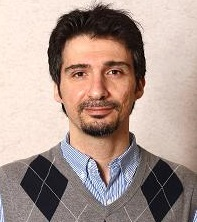
\includegraphics[width=1in,height=1.25in,clip,keepaspectratio]{./images/kamer.jpg}}]{Kamer Kaya} is an Assistant Professor at the Faculty of Engineering and Natural Sciences at Sabancı University. He got his PhD from Dept. Computer Science and Engineering from Bilkent University. He worked at CERFACS, France, as a post-graduate researcher in the Parallel Algorithms Project. He then joined the Ohio State University in September 2011 as a postdoctoral researcher, and in December 2013, he became a Research Assistant Professor in the Dept. of Biomedical Informatics.
His current research interests include Parallel Programming, High Performance Computing, and Cryptography. 
    \end{IEEEbiography}

\end{document}


